\subsection {Global Address Space}
\label{sec:gas}

The global address space (GAS) view is essential to implement any PGAS
language like \Xten{}.\Xtenlib{} provides this abstraction for \Xten{}.
An address space (AS) is $k$-bits if it can support addresses from $0$
to $2^k-1$. We are concerned with two address spaces -- the Local
Address Space (LAS), representing the address space in a single process
running on an SMP, and the Global Address Space (GAS), representing the
entire address space available to the computation, i.e. collection of
processes, scattered on multiple SMPs. The LAS is divided in two regions
-- private and shared.


\begin{figure}
\center
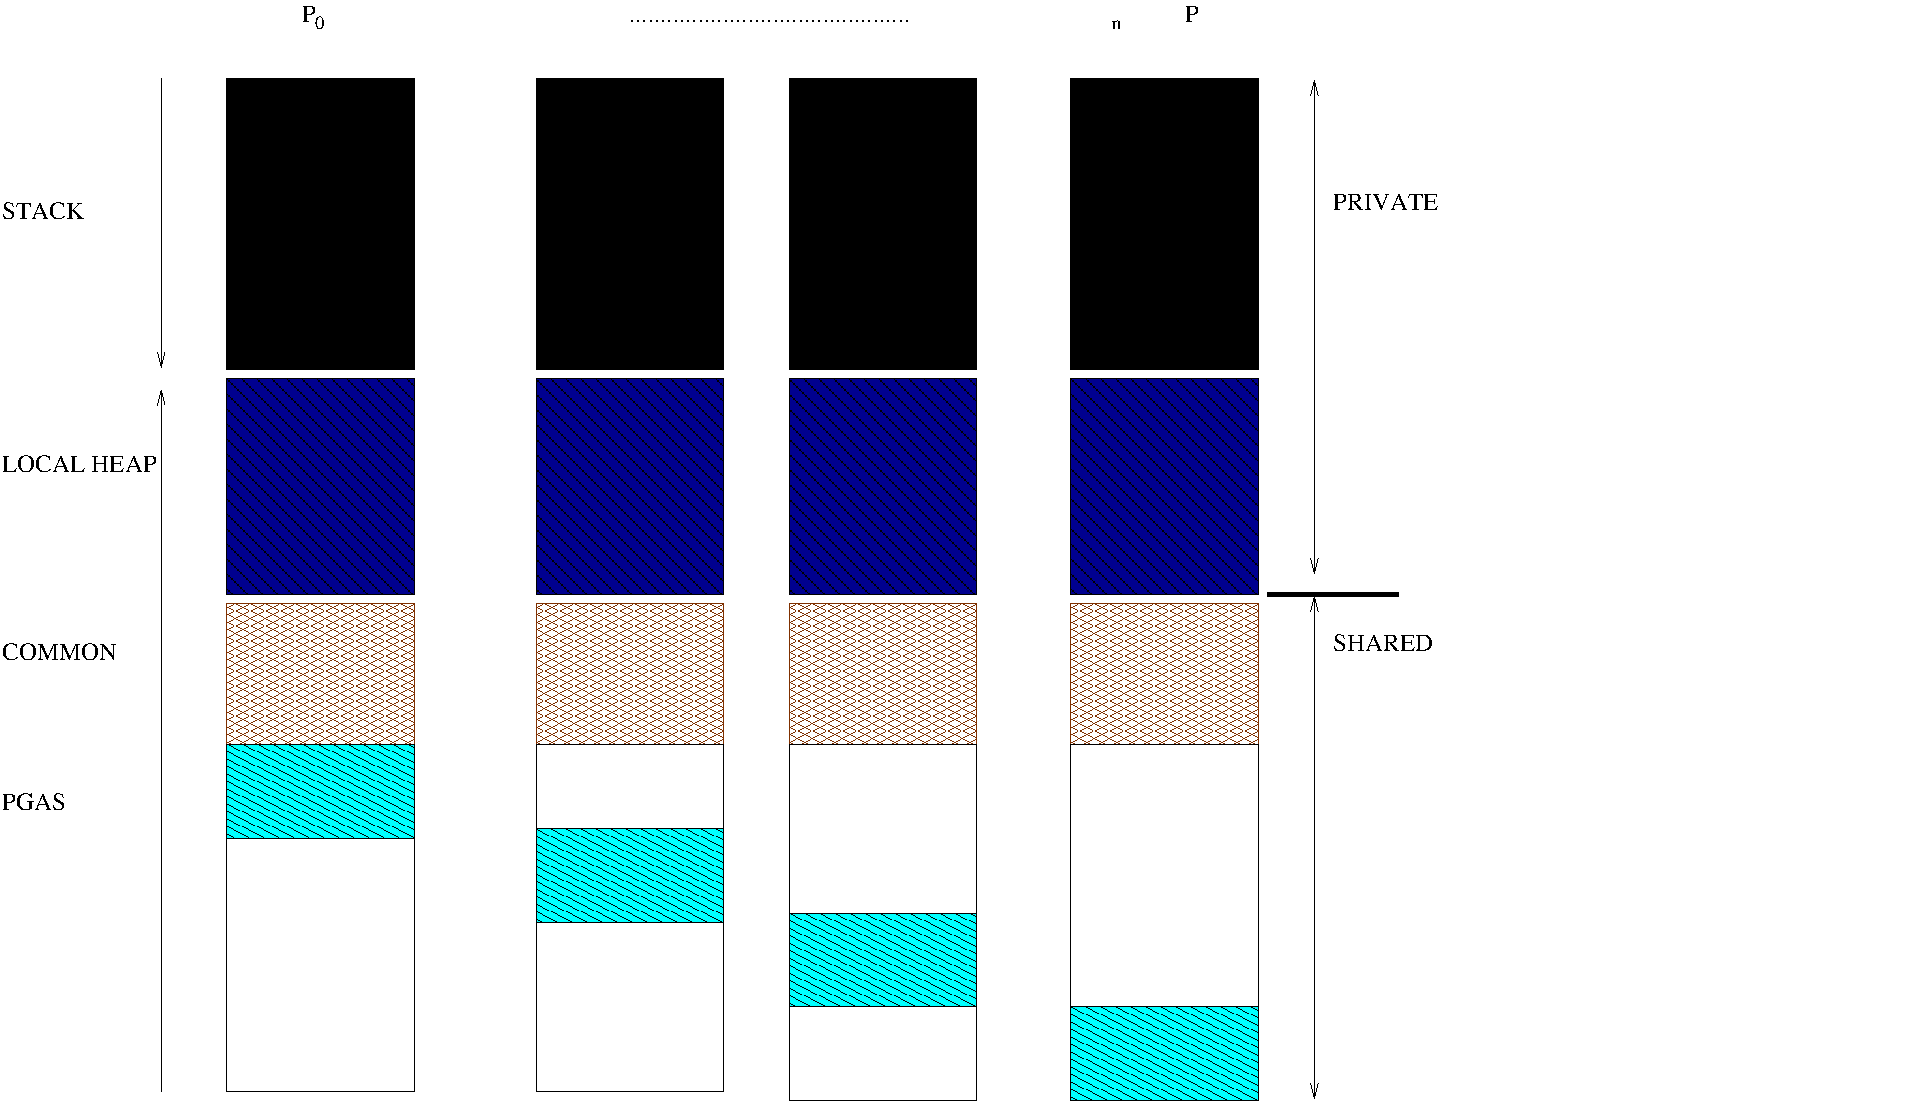
\includegraphics[scale=0.5]{figs/gas.pdf}
\caption{\Xten{} The address space of an \Xtenlib{} process}
\label{fig:as_layout}
\end{figure}

The shared region of a process is divided in two -- {\em common} and
{\em hosted}. The higher $n$-bits of the 64-bit address (i.e. $a_{63-x}$
to $a_{63-x-n}$) are used to address the common section. Each process
stores its meta-data pertaining to global data structures in the common
section. For example, the meta-data (region, distribution, base address)
of a distributed array are stored in the common section. Pointers to the
common address space can be locally dereferenced and memory locations
can be directly accessed.

Now we divide up the remaining address space among the $2^p$ nodes by
using the next $p$ higher-order bits (ie. $a_{63-x-n-1}$ to
$a_{63-x-n-p}$). The portion of the address space that is allocated to a
given processor $P$ is said to be ``hosted'' at $P$. We call the union
of the address spaces hosted at each processor the ``partitioned address
space.'' Thus the total shared address space is divided up into the
partitioned address space and the common address space. The entire
address space is pictorially represented in Figure~\ref{fig:as_layout}. 

Whenever a processor $P$ desires to read or write an address  $A$ in the 
partitioned address space, it first determines the processor $Q$ at which 
this address is hosted, and then asks $Q$ to read or write the address on 
its behalf (using LAPI remote gets and puts). Note that  $A$ is valid in 
$P$'s address space but will never be referenced. So $P$'s virtual memory 
tables will need to allocate real memory only to the portion of the 
address space that is hosted at $P$ or is common.

An advantage of such a representation is that address arithmetic can be 
performed locally. Suppose that a processor wishes to get the contents 
of $A[i]$. The code will read the metadata for $A$ from locations in the  
Common Address Space. Using this information (e.g.{} information that says 
the array is block distributed, and provides the block size), the code 
will compute the target address for $A[i]$. Note that the code sequence 
necessary to do this calculation is {\em identical} across all nodes. Now 
that the target address is known the code will determine whether it is 
local or remote by examining the higher order bits. If it is local then 
it reads the location from its local memory, otherwise it uses a 
LAPI-get to read the memory.

%It is not required that the contents of memory in the common address
%space are actually identical across all processors.  Often they will
%be. But sometimes they will be different. For instance, in the case of
%global array A, the meta-data will be stored in the common
%address space. The first (64-bit) word at this address will contain a pointer
%into the portion of the partitioned address space hosted at this node
%which contains the data for the local portion of the array.
%Subsequent words may contain the meta-data for the array -- the
%contents of these words may be identical across all nodes.

Addresses in the Common Address Space ``mean'' the same to all
processors, e.g. the global array A represented by the address
0x000078ABCDDDDDD in the Common Address Space. So processor $P$ can send
a message to any other process $Q$ with this address, and $Q$ will be
able to use it to get to its local data for $A$. The contents of the
first word at this address will be {\em different} for each processor
$Q$ -- but will mean ``the same,'' i.e the local portion of the array.

\subsubsection {GAS Implementation}

The new operator in C++ should be overloaded and thus transparently
(i.e. without explicitly telling at an allocation site) use a custom
memory allocator for objects of certain types.  A sufficiently large
chunk of the address space is allocated ahead of time using a special OS
call (e.g. {\bf mmap}). The distributed objects and arrays are placed in
this large chunk as the program executes.  The custom memory allocation
for PGAS implementation (done in C++ or C) is useful for two reasons.

First, depending on the communication subsystem (e.g. LAPI) virtual
memory pages that belong to the PGAS may have to 'pinned', i.e. marked
to stay resident in main memory. This is necessary to serve remote
accesses timely without the risk that a remote access hits into virtual
memory that is paged out. 

Secondly, one can allocate the chunks of a distributed array in
different nodes at the same address offset. If both contiguous array
variables are allocated at the same offset in the virtual address space
in each node, then the computation of the virtual address of any array
variable can be done easily at the source node without any address
translation at the home node.

\subsubsection {Remote References}

In shared memory systems where all accesses to data are through global
pointers, all pointers are valid at all places. In such a scenario,
the programmer can separate the problems of data distribution and
computation partitioning. This greatly simplifies programming. In a
distributed memory machine the shared memory abstraction incurs a
performance penalty. This can be reduced by automatically translating
global pointers to local pointers where possible.  In the context of
\Xten, every pointer carries the place of residence in its type. The
compiler can translate global reference to local references. Asyncs
that are thus determined to operate on local pointers can be inlined.

The runtime does not provide any such support and requires the user to
explicitly distinguish local and remote references. In \Xtenlib, remote
references encapsulate global pointers, potentially making them
safer. In a typical one-sided library, global pointers are identified
by a place id and a pointer at that place. These two components are
visible at all places, potentially allowing dereference of a remote
pointer at the current place, resulting in undefined behavior.

\Xtenlib{} allows access to the pointer encapsulated by a global pointer,
only if that global pointer is local, i.e., points to a data structure
at the current place. This prevents accidental dereference of the
global pointer at an incorrect place. To access an address that is not
local (i.e. read or write), LAPI put/get methods should be used. 
